\documentclass[border=4pt]{standalone}
\usepackage{tikz}
\usepackage{pgfplots}
\pgfplotsset{compat=1.18}
\usetikzlibrary{shapes.geometric,arrows.meta,positioning,calc,fit,decorations.pathreplacing,backgrounds}
\definecolor{boxblue}{RGB}{225,238,252}
\definecolor{boxgreen}{RGB}{225,247,231}
\definecolor{boxorange}{RGB}{253,236,216}
\definecolor{boxgray}{RGB}{237,237,237}
\definecolor{boxred}{RGB}{253,226,226}
\begin{document}
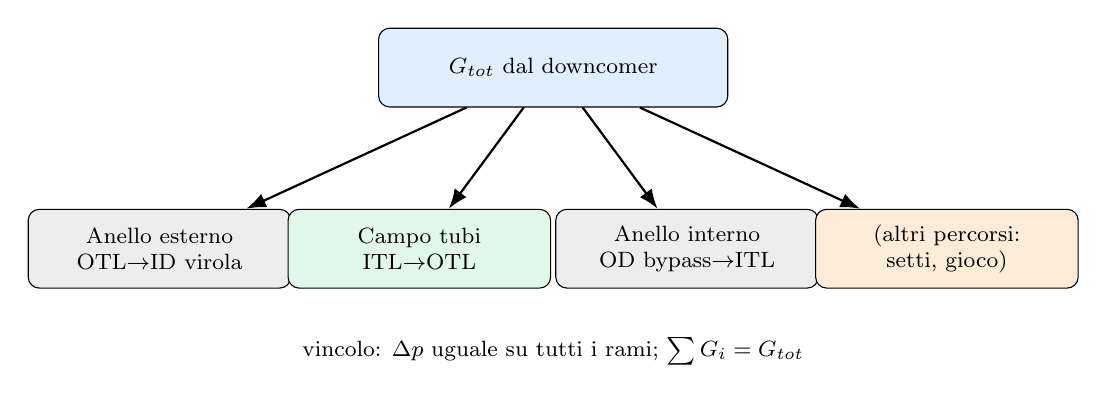
\begin{tikzpicture}[
  box/.style={draw, rectangle, rounded corners, minimum height=1.0cm, text width=3.1cm, align=center, font=\footnotesize},
  arr/.style={-{Latex[length=2.5mm]}, thick}
]
\node[box, fill=boxblue, text width=4.2cm] (src) at (0,1.7) {$G_{tot}$ dal downcomer};
\node[box, fill=boxgray] (r1) at (-5.0,-0.6) {Anello esterno\\ OTL$\to$ID virola};
\node[box, fill=boxgreen] (r2) at (-1.7,-0.6) {Campo tubi\\ ITL$\to$OTL};
\node[box, fill=boxgray] (r3) at (1.7,-0.6) {Anello interno\\ OD bypass$\to$ITL};
\node[box, fill=boxorange] (r4) at (5.0,-0.6) {(altri percorsi:\\ setti, gioco)};
\node[font=\footnotesize] at (0,-1.9) {vincolo: $\Delta p$ uguale su tutti i rami; $\sum G_i = G_{tot}$};
\draw[arr] (src) -- (r1); \draw[arr] (src) -- (r2);
\draw[arr] (src) -- (r3); \draw[arr] (src) -- (r4);
\end{tikzpicture}
\end{document}
